\renewcommand*{\arraystretch}{1.1}

\subsection*{BI / read / 18}
\label{section:bi-read-18}

\noindent\begin{tabularx}{\queryCardWidth}{|>{\queryPropertyCell}p{\queryPropertyCellWidth}|X|}
	\hline
	query & BI / read / 18 \\ \hline
%
	title & How many persons have a given number of posts
 \\ \hline
%
	pattern & \hfill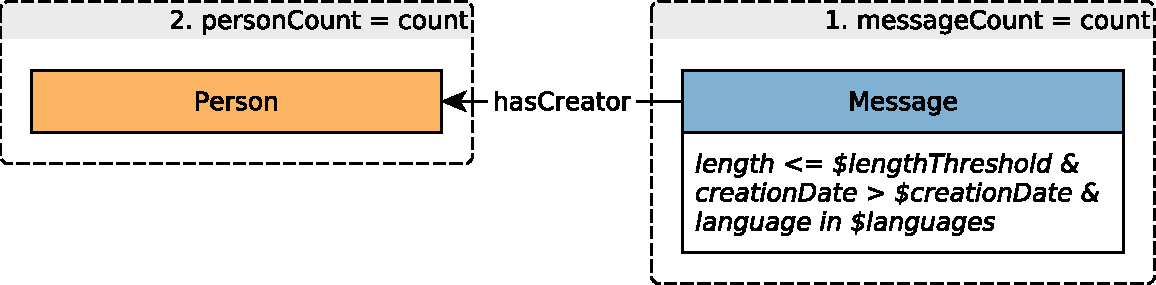
\includegraphics[scale=\patternscale,margin=0cm .2cm]{patterns/bi-read-18}\hfill\vadjust{} \\ \hline
%
	desc. & For each \emph{Person}, count the number of \emph{Messages}
(\emph{Posts} \& \emph{Comments}) they made.

Only consider messages with:

\begin{itemize}
\tightlist
\item
  length below the \texttt{lengthThreshold}
\item
  creationDate after \texttt{date} (exclusive, equality is not allowed)
\item
  any of the given \texttt{languages}
\end{itemize}

The language of a \emph{Comment} is that of the \emph{Post} that
initiates the thread where \emph{Comment} belongs to.
 \\ \hline
%
	
		params &
		\innerCardVSpace{\begin{tabularx}{\attributeCardWidth}{|>{\paramNumberCell}c|>{\varNameCell}M|>{\typeCell}m{\typeWidth}|Y|} \hline
		$\mathsf{1}$ & date
 & Date
 &  \\ \hline
		$\mathsf{2}$ & lengthThreshold
 & 32-bit Integer
 &  \\ \hline
		$\mathsf{3}$ & languages
 & String{[}{]}
 &  \\ \hline
		\end{tabularx}}\innerCardVSpace \\ \hline
	
%
	
		result &
		\innerCardVSpace{\begin{tabularx}{\attributeCardWidth}{|>{\resultNumberCell}c|>{\varNameCell}M|>{\typeCell}m{\typeWidth}|>{\resultOriginCell}c|Y|} \hline
		$\mathsf{1}$ & messageCount & 32-bit Integer & A &
				Number of \emph{Messages} created
 \\ \hline
		$\mathsf{2}$ & personCount & 32-bit Integer & A &
				The number of \emph{Persons} with \texttt{messageCount} messages
 \\ \hline
		\end{tabularx}}\innerCardVSpace \\ \hline
	
%
	
		sort		&
		\innerCardVSpace{\begin{tabularx}{\attributeCardWidth}{|>{\sortNumberCell}c|>{\varNameCell}M|>{\directionCell}c|Y|} \hline
		$\mathsf{1}$ & personCount
 & $\desc
$ &  \\ \hline
		\end{tabularx}}\innerCardVSpace \\ \hline
	%
	%
	CPs &
	\multicolumn{1}{>{\raggedright}l|}{
		\chokePoint{1.1}, 
		\chokePoint{1.2}, 
		\chokePoint{1.6}, 
		\chokePoint{3.2}, 
		\chokePoint{4.2}, 
		\chokePoint{4.3}
		} \\ \hline
	%
	%
\end{tabularx}
\queryCardVSpace